% Following magic comments allow for compilation of root file
% !TEX root = ../../../../temp_manuscript.tex

\chapter{Introduction}

\section{Glioma}

When cells reproduce, genetic changes can occur that might cause the cells to grow uncontrollably.
This uncontrollable growth of new cells is commonly known as cancer.
When the cancerous cells clump together, the single mass that they form is called a tumour.
Tumours can originate from and occur in almost every anatomical location, and the location where the tumour occurs does not have to be the same as the location from which the cancerous cells originated.
When the tumour appears in the same anatomical location as the anatomical origin of the cells, the tumour is called a primary tumour.
Hence, primary brain tumours are tumours located in the brain that are formed by cells that mutated from (healthy) brain cells.

Since different types of brain cells exist, the cancerous cells can have evolved from these different cells.
Therefore, primary brain tumours are categorized by the type of brain cells from which they originated, with gliomas being the most prevalent type \autocite{leece2017indicence}.
Gliomas originate from glial cells, which play a supporting role in the central nervous system and are the most abundant cell type in the brain \autocite{jakel2017glial}.
Although gliomas have a low incidence compared to other cancers, around \per{1.7} globally \autocite{leece2017indicence}, they are quite lethal with a median survival of around ten months \autocite{hess2004gliomaincidence}.

\section{Glioma categorization}
Historically gliomas were categorized based solely on their histological appearance, that is the appearance of the tumour cells under a microscope.
Up to 2016, the \gls{WHO} recognized four different types of glioma: astrocytoma, oligoastrocytoma, oligodendroglioma, and glioblastoma.
This classification depended on the type of glial cells that were visible in the tumour tissue \autocite{louis2007who}.
In addition to the glioma type, tumours were assigned a grade to indicate the aggressiveness of the tumour.
The grade was either II, III, or IV, with a grade IV glioma being the most aggressive.
Glioblastoma are grade IV glioma, while astrocytoma, oligoastrocytoma, and oligodendroglioma could be either grade II or grade III.

However, this categorization based on the glial cell type and the grade was suboptimal.
Firstly, the histological categorization and grading of the tumours are very observer-dependent \autocite{mittler1996gradingreliability, vandenbent2010interobserver}.
Since the clinical decision making depended on these categorizations, this observer-dependency can lead to a inadequate treatment of the tumour \autocite{vandenbent2010interobserver}.
Secondly, within these categories, large differences between the survival of patients existed, suggesting a different underlying mechanic at play \autocite{dubbink2015molecular}.
For example, some grade III glioma showed survival rates that were more characteristic of grade IV glioma than other grade III glioma.
It was found that this difference can be explained by the genetic features of the tumour \autocite{dubbink2015molecular,eckel2015gliomagroups}.
Therefore, in 2016 the \gls{WHO} updated the categorization of glioma to include these molecular features \cite{louis20162016} and depend less on the histology alone.
This update led to better patient stratification and more objective categorization of the glioma \autocite{molinaro2019geneticepidemiology}.

The WHO 2016 classification recognized two important genetic markers:  the \gls{IDH} mutation and \acl{1p19qcotion}.
Furthermore, the histological classification is also simplified.
The difference between astrocytoma, oligoastrocytoma, oligodendroglioma, and glioblastoma is no longer relevant.
The histology only needs to recognize the astrocytoma, oligoastrocytoma, oligodendroglioma on one hand or glioblastoma on the other hand.
This greatly reduces the inter-observer variability as most variability was observed in distinguishing between astrocytoma, oligoastrocytoma, and oligodendroglioma \autocite{mittler1996gradingreliability}.
An overview of the \gls{WHO} 2016 guidelines is presented in \cref{fig:intro_glioma_categorization}.


\begin{figure}[hbt]
    \resizebox{0.8\textwidth}{!}{\subimport{Figures/}{WHO_2016_flowchart.pgf}}
    \centering
    \caption{The WHO 2016 categorizaton of glioma.}\label{fig:intro_glioma_categorization}
\end{figure}


Within the grade II and grade III glioma (the astrocytoma, oligoastrocytoma, and oligodendroglioma), the following categories now exist:

\begin{itemize}
    \item Diffuse astrocytoma, \gls{IDH} wildtype
    \item Diffuse astrocytoma, \gls{IDH} mutated
    \item Oligodendroglioma, \gls{IDH} mutated and 1p/19q codeleted
\end{itemize}

No category exists for 1p/19q co-deleted, \gls{IDH} wildtype glioma since it has been found that all 1p/19q co-deleted tumors are also IDH mutated \autocite{labussi20101p19qcodeletedIDH}. The oligodendroglioma group has the best prognosis in these group, with the diffuse astrocytoma IDH wildtype showing the worst prognosis.
Due to the aggressiveness of IDH wildtype astrocytoma, it is even suggested that these are actually misclassified glioblastoma \autocite{hartmann2010IDH1gbm, brat2018IMPACT}.

The \gls{WHO} 2016 guidelines also categorize \gls{GBM} based on the \gls{IDH} mutation status, with \gls{IDH} mutated \gls{GBM} having a better prognosis than \gls{IDH} wildtype \gls{GBM}.
Although the guidelines currently only recognize the \gls{IDH} mutations status, there is another genetic feature that plays an important role in \gls{GBM}: \gls{MGMT} methylation.
\gls{MGMT} methylation is an important molecular marker, where patients with \gls{MGMT} methylation survive longer \autocite{martinez2007MGMT, gessler2018MGMT, weller2009molecularGBM}.
Thus, although not officially part of the most recent \gls{WHO} guidelines the \gls{MGMT} methylation status is now often also taken into account during the clinical decision making \cite{molinaro2019geneticepidemiology}.

Not only is there a difference in the prognosis of the tumours depending on their molecular features, but tumours also respond differently based on their genetic features.
For example \gls{IDH} mutated glioma respond better to radiotherapy \autocite{juratli2015IDHtreatment}, whereas the 1p19q co-deletion status and MGMT methylation status might be predictors of the sensitivity to chemotherapy \autocite{idbaih2007markersresponse}.
Thus, it is important to know the genetic subtype of the glioma, both for the prognosis of the patient as well as for the treatment plan.

In current clinical practice, the genetic features are determined either from a biopsy, or a resection.
In the case of a biopsy, a small part of the tumor is removed for analysis.
Resection is usually part of the treatment process, and involves removing as much of the tumour as possible.
Part of the removed tumour can then be used for the genetic and histopathological analysis.
Taking a biopsy and resecting the tumour both require intrusive surgery, which can negatively impact the patient.
Therefore, it would be beneficial if the molecular status of a glioma could be determined without the need for a biopsy or resection.
This is especially relevant in the case of a biopsy since the sole purpose of the biopsy is to obtain tissue that can be analyzed to help the clinical decision making.

Having a non-invasive method to determine the genetic features of the tumour not only obviates the need for an intrusive surgical operation, but it also provides relevant information earlier in the treatment process which can aid in the clinical decision making.
In some cases, especially for the 1p/19q co-deleted, IDH mutated oligodendroglioma, it might be better to follow a watch-and-wait approach since leaving tumour might have less of a negative impact than the potentially damaging effect of the treatment \autocite{vandenbent2012lggtreatment, welle2017EANO}.
Since \gls{MRI} is already part of the standard clinical pathway for glioma patients, the question quickly arose whether it was possible to use the radiological imaging as a non-invasive alternative to identify the genetic features of the tumour.

\section{Radiological analysis of glioma}

\gls{MRI} is an imaging technique that uses the magnetic property of protons, one of three elementary particles that form an atom, to create an image.
Although protons appear in all atoms, hydrogen atoms are of particular interest because they consist of a single proton and thus can easily be manipulated.
Furthermore, a water molecule contain two hydrogen atoms and since the majority of the body consists of water hydrogen atoms (and thus protons) are abundant in the human body, especially in tissue.
The magnetic properties of the protons arise from their \say{spin}, a quantum mechanical property that can be compared to a spinning top that spins around its own axis.
Normally the spins of the protons are distributed randomly, which means that they cancel each other out and thus nothing can be measured.
However, by applying an external magnetic field the spins can be forced to all point in the same direction.
Once the spins are all aligned it is possible to excite the spins by applying a magnetic field in a different direction for a short time.
Then measuring how long it takes for the spins to go back to their resting state can be used to create an image.
By exciting the spins in different ways, it is possible to obtain different \say{image contrasts} that show different properties of the tissue.

\gls{MRI} is routinely being used in clinical care, since it can be used to distinguish between healthy and diseased tissue.
Shortly after the first introduction of \gls{MRI}, it was proposed that the method could be used to identify tumors \autocite{damadian1971tumor}.
After some improvements, the technique was first applied to the brain in 1980 \autocite{holland1980brain}, and in the same year MRI has first been used to investigate a possible tumor in the brain.
Since then quality of \gls{MRI} scans has vastly increased, and different \gls{MRI} techniques have been developed that can image different tissue characteristics.
\cref{fig:intro_MR_modern} shows some of the currently most popular imaging sequences, although many others exist.
Here the tumor can clearly be seen in the patients brain, and therefore \gls{MRI} is now the standard-of-care for brain tumor diagnosis and treatment decisions.

\begin{figure}[hbt]
    \centering
    \begin{subfigure}[b]{0.45\textwidth}
        \centering
        \includegraphics[width=\textwidth]{example-image-a}
        \caption{First scan of a human glioma}\label{fig:intro_MR_first}
    \end{subfigure}
    \begin{subfigure}[b]{0.45\textwidth}
        \centering
        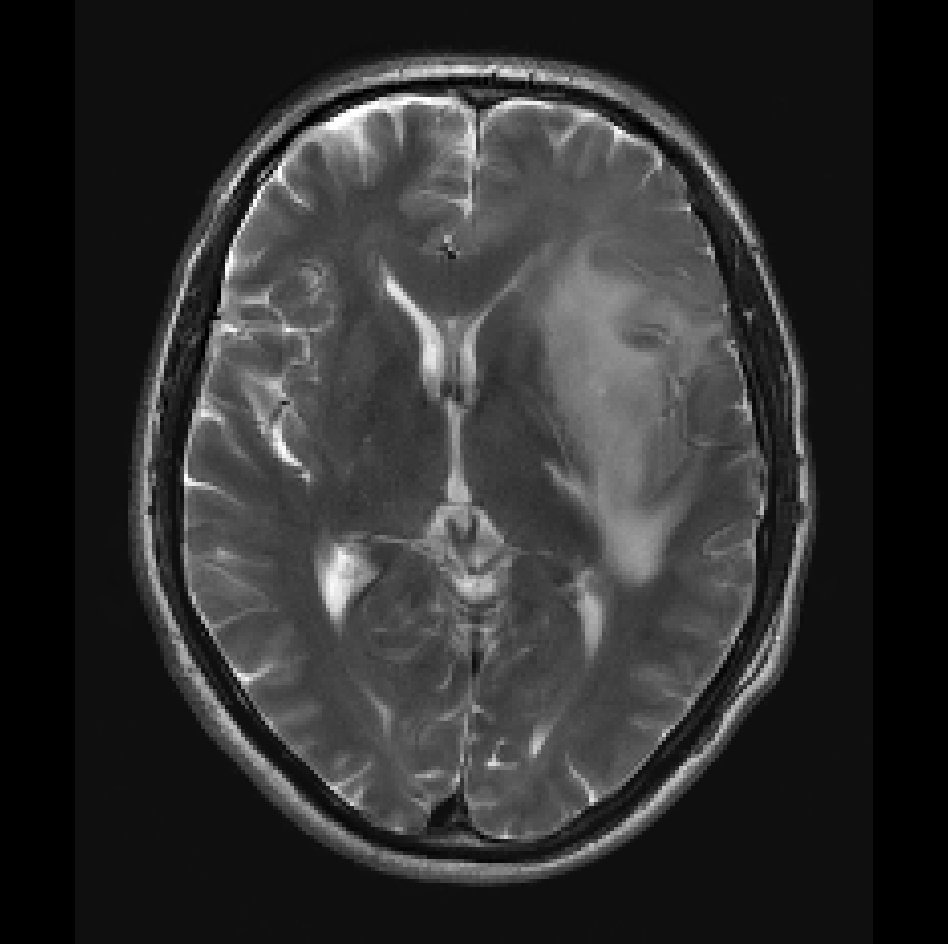
\includegraphics[width=\textwidth]{Figures/T2_LGG.png}
        \caption{Modern glioma scan}\label{fig:intro_MR_modern}
    \end{subfigure}
    \caption{\acrshort{MRI} scan of a glioma from 1980 and a recent \acrshort{MR} scan, showing the large improvement over time. On the modern scan the glioma can easily be identified}\label{fig:intro_MR_comparison}
\end{figure}

\gls{MRI} scans are already routinely being used to get a first indication of the aggressiveness of the tumor, mainly for the evaluation of the grade \autocite{upadhyay2011MRIevaluation}.
With the increasing importance of genetic markers of the tumors, research has focused on identifying imaging features that correlate with the status of the genetic markers of a tumor \autocite{patel2017mismatch, smits2016imaging}.
These imaging features that correlates with an underlying physiological aspect are called imaging biomarkers.
The presence of these biomarkers is a promising non-invasive alternative to tumor biopsy and resection.
However, the use of imaging biomarkers is not without problems.

Firstly, \gls{MRI} is a qualitative and not a quantitative measurement, meaning that there is a large difference between scans of the same patient on different machines, and sometimes even on the same machine.
This makes it hard to define a proper measurement value from an \gls{MR} scan, and thus to define a robust method that can easily be broadly applied.
Secondly, most biomarkers are rather simple; looking at a single point in the tumor or only considering the 2D measurements of a tumor.
Methods are kept simple so that they can easily be used by the clinician and do not require complicated, time-consuming measurement.
However, this limits the amount of information that such a method can take into account, thus pressing on the performance of these methods.
Because of these restrictions biomarkers to be used by clinical experts are often vaguely defined and are not objective.
Thus, the proper measurement of these imaging biomarkers also relies on the expertise of the treating physician, causing a large inter- and intra-observer variability in the measurements.
This makes it difficult to broadly apply a method, causes a drop in performance and results in the patient treatment being dependent on the treating physician.
Thus, a method that would be more objective and consistent, that can take into account complex relationships of the image, while not being too complex and time-consuming for the clinician to use is needed.

This demand was met by the field of machine learning.
Although the exact definition of \say{machine learning} differs from person to person, in general machine learning methods are methods that leverage (large amounts of data) to find common patterns and uses these patterns to classify the data.
For example, one can make an algorithm and provide it with pictures of cats and dogs, from which the algorithm then has to learn which pictures are cats and which pictures are dogs.
A lot of different machine learning methods exist, but one way of separating the methods is by whether they use human-defined features or determine features themselves.
When a method uses human-defined features it is possible to feed it with imaging biomarkers that have been previously discovered.
On the other hand some machine learning methods can learn relevant features directly from the raw data, allowing for possibly better features.

Using a computational method removes (part of) the human element of measurements, it will be more consistent (when the same patient is presented multiple times it will give the same output), and depending on the method can take into account complex relationships in the data.
Of course this comes at a price, mainly at the cost of interpretability.
Since the method can find complex relationships, it might is then difficult to understand why a method made a certain decision.
However, the high performance of these methods and the other advantages have caused them to now be routinely used.
In the biomedical imaging field machine learning methods are often used to classify images as disease vs healthy or to classify the state of a disease.
This area of research is called \say{radiomics}, where a subfield which focuses on predicting the genetic markers based on imaging is called \say{radiogenomics}.
In the (neuro-)oncology fields radiogenomics quickly gained in popularity, largely due to the WHO 2016 redefinition which was now based on the genomic status.
An in-depth introduction of machine learning, radiomics and the different methods is given in \cref{chap:radiomics}.


Say something about automated methods outside of machine learning


Using machine learning and other automated methods allows for a larger availability of information, which a clinician can use for the diagnosis and treatment decision of a patient.

\section{Thesis outline}
Therefore, in this research we investigate different methods with which we can gain more insight into gliomas from MR imaging. This thesis has three main goals:
\begin{itemize}
\item Add to the knowledge of biomarkers of glioma, which experts can use to evaluate new patients
\item Automate analysis of glioma MR imaging to provide information about the clinical characteristics of the tumor
\item Provide automated tools and structured data to make glioma MR research available to a broader public more quickly.
\end{itemize}

The thesis is structured as follows:

In \cref{chap:radiomics} introduce the concept of machine learning and radiomics and detail the different terms used, as well the proper way to carry out such experiments.

In \cref{chap:LGGLocation} and \cref{chap:HGGLocation} there is a focus on the relationship between the molecular status of glioma and their location in the brain.
Here we investigate whether from the location of the tumor it is possible to say something about the (likely) molecular status, and thus whether the location of the glioma is a biomarker.

In \cref{chap:LGG1p19q} I use a machine learning method to predict the 1p/19q co-deletion status of low grade glioma.
Here we show that it is possible to automate this task, and that our method also extends to a different independent set.
We also present some biomarkers that our method found and showed that these have similarities with known biomarkers from literature.

In \cref{chap:discussion} I discuss the results from all the previous chapter and explore the possibilities for future directions.

